\documentclass{beamer}

% Theme
\usetheme{Madrid}
\usecolortheme{default}

% Packages
\usepackage{amsmath,amssymb,amsfonts}
\usepackage{graphicx}
\usepackage{xcolor}
\usepackage{tikz}
\usepackage{tkz-euclide}
\usepackage{array}
\usepackage{multirow}
\usepackage{longtable}
\usepackage{lscape}
\usepackage{listings}
\lstset{
    basicstyle=\ttfamily\small,
    keywordstyle=\color{blue},
    commentstyle=\color{gray},
    stringstyle=\color{red},
    showstringspaces=false,
    breaklines=true
}



% Custom macros
\newcommand{\myvec}[1]{\begin{pmatrix}#1\end{pmatrix}}
\newcommand{\brak}[1]{\left( #1 \right)}

% Redefine \vec to bold letters only (no arrow)
\renewcommand{\vec}[1]{\mathbf{#1}}

\title{2.4.13}
\author{EE25BTECH11019 -- Darji Vivek M.}
\date{}

\begin{document}

% Title slide
\begin{frame}
  \titlepage
\end{frame}

% Question slide
\begin{frame}{Question}
$\vec{B}-\vec{A}=3\vec{i}-\vec{j}+\vec{k}$ and $\vec{D}-\vec{C}=-3\vec{i}+2\vec{j}+4\vec{k}$ are two vectors.  
The position vectors of the points $\vec{A}$ and $\vec{C}$ are $6\vec{i}+7\vec{j}+4\vec{k}$ and $-9\vec{j}+2\vec{k}$, respectively.  
Find the position vectors of a point $\vec{P}$ on the line $\vec{A}\vec{B}$ and a point $\vec{Q}$ on the line $\vec{C}\vec{D}$ such that $\vec{Q}-\vec{P}$ is perpendicular to both $\vec{B}-\vec{A}$ and $\vec{D}-\vec{C}$.  
\hfill $\brak{10,2021}$
\end{frame}

\begin{frame}{Solution: Variables Used}
\small
\begin{table}[h!]
    \centering
    \begin{tabular}{|c|c|}
        \hline
        Point & Coordinates \\
        \hline
	    $A$ & $\myvec{1\\-1}$ \\
	    $B$ & $\myvec{-4\\2k}$ \\
	    $C$ & $\myvec{-k\\-5}$ \\
        \hline
    \end{tabular}
    \caption{Vertices of $\triangle ABC$ before substituting $k$}
    \label{tab:triangle_k}
\end{table}

\end{frame}

\begin{frame}{Solution: Matrix Method}
\small
Points on the lines can be written as
\[
\vec{P}=\vec{a}+\lambda\vec{d}_1, \qquad
\vec{Q}=\vec{c}+\mu\vec{d}_2
\]

Then
\[
\vec{Q}-\vec{P}=(\vec{c}-\vec{a})+\mu\vec{d}_2-\lambda\vec{d}_1
\]

Perpendicularity to both $\vec{d}_1$ and $\vec{d}_2$ gives
\[
\vec{d}_1^{\top}(\vec{Q}-\vec{P})=0, \qquad
\vec{d}_2^{\top}(\vec{Q}-\vec{P})=0
\]

This yields the $2\times 2$ linear system
\[
\begin{bmatrix}
11 & -7 \\ 
-7 & 29
\end{bmatrix}
\begin{bmatrix}
\lambda \\ \mu
\end{bmatrix}
=
\begin{bmatrix}
4 \\ 22
\end{bmatrix}
\]
\end{frame}

\begin{frame}{Solution: Computation}
\small
Solving:
\[
\lambda=-1,\qquad \mu=1
\]

Therefore,
\[
\vec{P}=\vec{a}+\lambda\vec{d}_1
=\begin{bmatrix}6\\7\\4\end{bmatrix}+\left(-1\right)\begin{bmatrix}3\\-1\\1\end{bmatrix}
=\begin{bmatrix}3\\8\\3\end{bmatrix}
\]

\[
\vec{Q}=\vec{c}+\mu\vec{d}_2
=\begin{bmatrix}0\\-9\\2\end{bmatrix}+1\cdot\begin{bmatrix}-3\\2\\4\end{bmatrix}
=\begin{bmatrix}-3\\-7\\6\end{bmatrix}
\]

Verification:
\[
\vec{Q}-\vec{P}=\begin{bmatrix}-6\\-15\\3\end{bmatrix}, \quad
\vec{d}_1^{\top}(\vec{Q}-\vec{P})=0,\quad
\vec{d}_2^{\top}(\vec{Q}-\vec{P})=0
\]
\end{frame}

% C Function
\begin{frame}[fragile]{C Function: Compute P and Q}
\begin{lstlisting}
#include <stdio.h>

// Function to compute P and Q points
void compute_points(double *Px, double *Py, double *Pz,
                    double *Qx, double *Qy, double *Qz) {
    double A[3] = {6, 7, 4};
    double AB[3] = {3, -1, 1};
    double C[3] = {0, -9, 2};
    double CD[3] = {-3, 2, 4};
    double lambda = -2, mu = -3;

    *Px = A[0] + lambda * AB[0];
    *Py = A[1] + lambda * AB[1];
    *Pz = A[2] + lambda * AB[2];

    *Qx = C[0] + mu * CD[0];
    *Qy = C[1] + mu * CD[1];
    *Qz = C[2] + mu * CD[2];
}
\end{lstlisting}

\end{frame}

% Python Code Beamer Slides
\begin{frame}[fragile]{Python: Load C Library}
\begin{lstlisting}[language=Python]
import ctypes
import numpy as np
import matplotlib.pyplot as plt

# Load shared C library
lib = ctypes.CDLL('./3.so')
lib.compute_points.argtypes = [ctypes.POINTER(ctypes.c_double),
                               ctypes.POINTER(ctypes.c_double),
                               ctypes.POINTER(ctypes.c_double),
                               ctypes.POINTER(ctypes.c_double),
                               ctypes.POINTER(ctypes.c_double),
                               ctypes.POINTER(ctypes.c_double)]
lib.compute_points.restype = None
\end{lstlisting}
\end{frame}

\begin{frame}[fragile]{Python: Call C Function}
\begin{lstlisting}[language=Python]
# Prepare variables
Px = ctypes.c_double()
Py = ctypes.c_double()
Pz = ctypes.c_double()
Qx = ctypes.c_double()
Qy = ctypes.c_double()
Qz = ctypes.c_double()

# Call C function
lib.compute_points(ctypes.byref(Px), ctypes.byref(Py), ctypes.byref(Pz),
                   ctypes.byref(Qx), ctypes.byref(Qy), ctypes.byref(Qz))

# Extract results
P = np.array([Px.value, Py.value, Pz.value])
Q = np.array([Qx.value, Qy.value, Qz.value])
print(f"P = {P}, Q = {Q}")
\end{lstlisting}
\end{frame}

\begin{frame}[fragile]{Python: Define Lines and Plot}
\begin{lstlisting}[language=Python]
# Given data
A = np.array([6, 7, 4])
AB = np.array([3, -1, 1])
C = np.array([0, -9, 2])
CD = np.array([-3, 2, 4])

# Generate line AB and CD
t = np.linspace(-5, 5, 100)
lineAB = A.reshape(3,1) + np.outer(AB, t)
lineCD = C.reshape(3,1) + np.outer(CD, t)

# Plot
fig = plt.figure()
ax = fig.add_subplot(111, projection='3d')

ax.plot(lineAB[0], lineAB[1], lineAB[2], label="Line AB")
ax.plot(lineCD[0], lineCD[1], lineCD[2], label="Line CD")
\end{lstlisting}
\end{frame}

\begin{frame}[fragile]{Python: Mark Points and PQ}
\begin{lstlisting}[language=Python]
# Points
ax.scatter(A[0], A[1], A[2], color='red', label='A')
ax.scatter(C[0], C[1], C[2], color='blue', label='C')
ax.scatter(P[0], P[1], P[2], color='green', label='P')
ax.scatter(Q[0], Q[1], Q[2], color='purple', label='Q')

# Connect PQ
ax.plot([P[0], Q[0]], [P[1], Q[1]], [P[2], Q[2]],
        'k--', label="PQ ⟂ AB,CD")

ax.legend()
plt.savefig("3.png")
plt.show()
\end{lstlisting}
\end{frame}


\begin{frame}{Python Output and Plot}
\begin{figure}[h!]
\centering
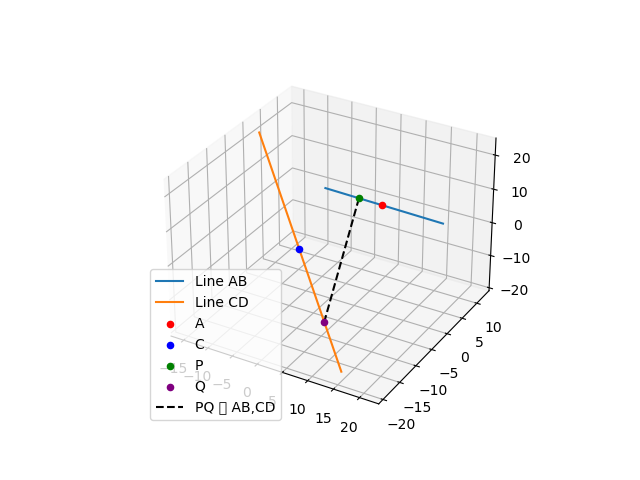
\includegraphics[width=0.75\columnwidth]{figs/3.png}
\caption{Perpendicular PQ between lines AB and CD computed via Python using C function.}
\end{figure}
\end{frame}

\end{document}
